\documentclass[a4paper,12pt,twoside]{report}

\makeatletter

	\usepackage[french]{babel}
	\usepackage[utf8]{inputenc}
	\usepackage[T1]{fontenc}
	
	
	\usepackage%
		{xcolor}
	
	\usepackage{xkeyval}
	\usepackage{geometry}
	\usepackage{graphicx}
	\usepackage{lipsum}
	\usepackage{xspace}			
	\usepackage{lmodern} 
    \usepackage{titling}
	\usepackage{sectsty}
	
	\usepackage{csquotes}


	
	\definecolorset{HTML}{}{}{belux,900A40;underbelux,AA526A;antibelux,000000}	% 
	
	
	\allsectionsfont{\color{black}}					
	\partfont{\color{belux}}						
	\chapterfont{\color{belux}}						
	\sectionfont{\color{belux}}						
	\subsectionfont{\color{belux}}					
	\subsubsectionfont{\color{underbelux}}				
	



%---------------------------
%% GEOMETRY MANAGEMENT

	\def\definegeometry#1#2{									%%
		\define@key{modelgeometries}{#1}[]{\geometry{#2}}			%%
		\define@key{setgeometrykeys}{#1}[]{\newgeometry{#2}}		%%
	}


	%%--------------------- \setmodelgeometry

	\newcommand{\setmodelgeometry}[1]{
		\setkeys{modelgeometries}{#1}
	}


	%%--------------------- setgeometry environment

	\newenvironment{setgeometry}[1]
		{\setkeys{setgeometrykeys}{#1}}
		{\restoregeometry}


	
	

	%% GEOMETRIES LIBRARY
	%%-------------------

	\definegeometry{math}			%% MATH
		{					
			inner=90pt,		
			bottom=65pt,
			top=65pt,
			outer=70pt			
		}
	
	\definegeometry{cover}			%% COVER - used in front_management
	{					
		top=3.5cm,			
		bottom=0cm,			
		inner= 0.6cm,		
		outer=0.6cm			
	}
	
	\setmodelgeometry{math}
	
	
\makeatother


%------------------
%------------------


%% PACKAGES
%\usepackage{caption,subcaption}
%	\captionsetup{singlelinecheck=off}

\usepackage{hhline}
\usepackage{eurosym}

\usepackage{tgcursor}

%%
\usepackage{appendix}
	\makeatletter
	%	\@addtoreset{chapter}{part}
		\@addtoreset{@ppsaveapp}{part}
	\makeatother

\usepackage[hidelinks]{hyperref}


\addto\captionsfrench{\renewcommand{\chaptername}{Partie}}


%\ExecuteBibliographyOptions{
%datamodel=NE_PAS_TOUCHER/mynote.dbx,
%}
\usepackage[
	%backend=biber,
 	style=numeric,
  	%citestyle=authoryear,
  	sorting=none,
    datamodel=NE_PAS_TOUCHER/mynote.dbx,
]{biblatex}
%\DeclareDatamodelFields[type=field,datatype=literal]{mynote}
\usepackage{xpatch}
\xapptobibmacro{finentry}{\par\printfield{mynote}}{}{}


%% COVER PREAMBLE


\usepackage{latexsym} % anciens symboles latex
\usepackage{makeidx}
\usepackage{calc}
\usepackage{ifthen}
\usepackage{float}
\usepackage{epsfig}
\usepackage{vmargin}
\usepackage{textpos}
\usepackage{color}
\usepackage{letterspace}
\usepackage{fancybox}

\setlength{\hoffset}{0cm}
\setlength{\voffset}{0cm}
\setlength{\paperheight}{29.7cm}
\setlength{\paperwidth}{21cm}
\setlength{\textwidth}{14.5cm}
\setlength{\marginparwidth}{0cm}
\setlength{\headheight}{2\baselineskip}
\setlength{\textheight}{21cm}
\setlength{\evensidemargin}{0cm}
\setlength{\oddsidemargin}{1.5cm}


%% Listings
\usepackage{listings}
\lstset{								% general command to set parameter(s)
	basicstyle=\ttfamily\small, 				% print whole listing small 
	keywordstyle=\color{black}\bfseries\underbar, 	% underlined bold black keywords 
	identifierstyle=, 					% nothing happens 
%	commentstyle=\color{white}, 				% white comments 
	stringstyle=\ttfamily, 					% typewriter type for strings 
	showstringspaces=false,
	numbers=left,
	numberstyle=\tiny\ttfamily,
	language=Java,
	tabsize=4,
	literate={{é}{{\'e}}1 {è}{{\`e}}1 {ê}{{\^e}}1 {à}{{\`a}}1 {œ}{{\oe}}1},
	xleftmargin=0pt,
	keywordstyle=\bfseries\color{underbelux},
	literate=							%
			{<-}{{$\leftarrow$}}{1}		%
			{<--}{{$\longleftarrow$}}{1}%
			{->}{{$\rightarrow$}}{1}	%
			{<->}{{$\leftrightarrow$}}{3}	%
			{-->}{{$\longrightarrow$}}{3}	%
			{<-->}{{$\longleftrightarrow$}}{4}	%
			{-|>}{{$\nrightarrow$}}{1}	%
			{+*}{{$\times$}}{1} 		%
			{A/}{{$\forall$}}{1}		%
			{é}{{\'e}}{1}				%
			{è}{{\`e}}{1}				%
			{ê}{{\^e}}{1} 				%
			{à}{{\`a}}{1}				%
			{É}{{\'E}}{1}				%
			{’}{{'}}{1}
	}


\lstdefinelanguage{pseudocode}
{
% list of keywords
morekeywords={
si, sinon, finsi, fsi, alors,
tantque, while, tant, que,
for, do, fintantque,fin, pour,
fonction, renvoyer, appeler,
TAD, fonctions, utilise, preconditions, 
booleen, entier
},
sensitive=false, % keywords are not case-sensitive
morecomment=[l]{//}, % l is for line comment
morecomment=[s]{/*}{*/}, % s is for start and end delimiter
morestring=[b]", % defines that strings are enclosed in double quotes
keywordstyle=\bfseries\color{darkgray}
}

\lstdefinelanguage{json}
{
	string=[s]{"}{"},
    stringstyle=\color{underbelux},
	morecomment=[l]{:},
	commentstyle=\color{black},
}


\newcommand{\displaycode}[2][]{\begin{center}\lstinline[mathescape,#1]^#2^ \end{center}}
	

%% DEFINITIONS


\def\cad{c'est-à-dire}
\def\ie{\emph{i.e.}}
	















\pretitle{\Huge \begin{center} \bfseries \color{belux}}
\title{Rapport de pré-étude \\[4mm] {Projet E-yaka}}
\date{\today}
\author{
	Raphaël \textsc{Esteveny} \and
	Quentin \textsc{Bigot} \and
	Pierre \textsc{Testart} \and
	Clément \textsc{Fournier} \and
	Jordan \textsc{Le Bongoat} \and
	Tom \textsc{Richardon} \and
	Arnaud \textsc{Cornillon} \and
	Jason \textsc{Barrier}
}
\widowpenalty10000
\setlength{\parskip}{4pt}

  \bibliography{CannabisPSH}
\begin{document}
	
		{
			\pagestyle{empty}
			\pagestyle{empty}
\fontfamily{cmss}
\selectfont

% LES DIFFERENTS CHAMPS DE LA COUVERTURE
\ordre{XXX}  % Le numéro d'ordre donné par le service de la recherche
\auteur{Prénom}{NOM}  % Prénom et nom de l'étudiant
\sautverticalnegatif{1.4} 
% Valeur en cm du saut vertical négatif (ie. vers le haut)
% Modifier cette valeur si le prénom et le nom de l'auteur ne sont pas positionnés au bon endroit par rapport à la ligne "Projet de Fin d'Etudes"
% Si le prénom et le nom tiennent sur la ligne, laisser valeur = 1.4
\specialite{XXX}  % Nom de la spécialité
\anneeuniversitaire{20xx - 20xx}  % Année universitaire
\titre{INTITULE DU PFE : le sujet qui peut s'écrire sur plusieurs lignes}  % sujet du PFE
\entreprisenom{Nom de l'entreprise}  % Nom de l'entreprise
\tuteur{Prénom}{Nom du tuteur}  % Prénom et nom du tuteur en entreprise
\correspondantINSA{Prénom}{Nom du correspondant INSA}  % Prénom et nom du correspondant INSA
\datesout{jj/mm/20xx}  % Date de la soutenance du PFE
\entrepriselogo{(Emplacement du logo de l'entreprise)}{terre}{1} 
% Remplacer le 1er paramètre "(Emplacement du logo de l'entreprise)" par un espace, le texte n'apparaîtra plus 
% Remplacer le 2ème paramètre "insaPFE" par le nom du fichier correspondant au logo de l'entreprise
% Ajuster le 3ème paramètre ici "1" par la largeur souhaitée (en cm) pour l'affichage du logo de l'entreprise
% S'il n'y a pas de logo à afficher, remplacer chacun des 3 paramètres par un espace
%
% RESUMES EN FRANÇAIS ET EN ANGLAIS
\resumefrancais{\textsf{Remplacer ce texte par le résumé en français}}
\resumeanglais{{Change this text by the abstract in english}}
% Les résumés en français et en anglais sont positionnés cote à cote 
% Une hauteur de cadre a été définie pour que les zones réservées aux résumés tiennent sur une seule page : ne pas la modifier 

\makepfe{insa}  % crée la couverture et la page avec les résumés (français et anglais)

	%		\cleardoublepage		
		}

\newgeometry{top=2cm,bottom=2cm,inner=3cm,outer=2cm}
	{
		\pagestyle{empty}
	%	\maketitle
		\tableofcontents
        \thispagestyle{empty}
        %\chapter*{Présentation synthétique}

\begin{abstract}
    ABSTRACT
\end{abstract}
		\listoffigures
        \begingroup
        \let\clearpage\relax
        \listoftables
        \endgroup
        \thispagestyle{empty}
		\cleardoublepage
	}
		
  			\chapter*{Introduction}
\addcontentsline{toc}{chapter}{Introduction}
\pagenumbering{arabic}


\addcontentsline{toc}{chapter}{\color{red}PROVISOIRE, n'hésitez pas à changer}

INTRO
			\chapter{Contexte du projet}



   			\chapter{Étude de l’existant}

    \section{Learning analytics}
    \section{MOOC}
    \section{Cahier des charges}
  			\chapter{Craindre des dérives ou se réjouir des bénéfices ?}

\section{Légaliser : vers un abus de la Beuh ?}

Tout comme pour de nombreuses substances nocives ou potentiellement nocives pour l’homme (alcool, café etc), le principal objectif du débat sur le cannabis est d’en réduire sa consommation parmi la population. Actuellement en France le cannabis est illégal, il est donc normal de se demander si sa légalisation n’entrainerait pas un abus de la beuh ; si autoriser l’interdit n’entraîne-t-il pas une hausse de sa consommation ?

\paragraph{Des similarités avec le cas de l'alcool ?}

 	Pour commencer, selon un rapport de l’ECDE (Organisation de coopération et de développement économiques) de mai 2015 sur les pratiques de \textit{binge drinking} (beuveries express) chez les jeunes \cite{oecd}, la facilité d’accès à l’alcool est une des raisons majeures de l’apparition et de la popularisation des dérives sur sa consommation. En effet ce rapport nous apprend par exemple que la part des garçons qui, à 15 ans, n’ont jamais bu d’alcool est passée de 44\% en 2001-02 à 30\% en 2009-10. La proportion de ceux qui à 15 ans ont déjà été ivres au moins une fois, est passée de 30\% à 43\% sur la même période. Des effets similaires sont présent chez les jeunes filles et avec cela des pratiques telle que le \textit{binge drinking} sont en augmentation. D’un autre côté, un rapport de l’IRDES (Institut de recherche et de documentation en économie de la santé) nous dit qu’en 2013, les ivresses chez les jeunes sont « plus fréquentes qu’en 2001 mais moins qu’en 1996 » \cite{irdes}. Nous voyons donc qu’il existe un possible « effet de mode générationnel » lui-même responsable dans les abus de consommation d’alcool mais il est évident que l’accessibilité de l’alcool seule est une source de dérives ; cela ne va-t-il pas être de même pour le cannabis ? 
    
    Globalement comme nous l’avons vu, le nombre de consommateurs réguliers de marijuana post-légalisation va dépendre du système dans lequel cette légalisation va être mise en place. Dans le scénario que nous trouvons comme étant le plus adapté, celui d’un monopole géré par l’État, ce nombre va probablement rester le même. En effet actuellement le cannabis est considéré comme étant très accessible pour un produit illégal : pour preuves le nombre important de consommateurs en France; son prix ---~fin 2014, le gramme de cannabis est en moyenne estimé à 6~\euro\ en France \cite{terraNova_rapport}; et l’avis de la population ---~en 2011, 43\% des adolescents français de 15-16 ans estimaient que, s’ils le voulaient, il leur serait « facile » d’obtenir du cannabis \cite{obradovic15}. \textit{Sa légalisation ne le rendrait donc pas beaucoup plus facilement atteignable}, et n’amènerait pas à un abus de sa consommation. 

\paragraph{Effet de mode/effet Streisand}

Nous pouvons ensuite également nous demander si cette légalisation ne créerait pas un effet de mode sur la marijuana. Cependant si « buzz » il y a, il ne serait que de courte durée et ne produirait une augmentation significative que du nombre de personne ayant testé au moins une fois le cannabis. À part cela, il n’existe pas de raisons pour que la légalisation rende la marijuana attractive sur le long terme. Au contraire, en étant illégal, le cannabis souffre d’un « effet Streisand » ---~ce qui est interdit attire~---, qui par définition est voué à disparaître en cas de légalisation. Pour expliquer ce phénomène d’effet Streisand, nous pouvons reprendre l’exemple de l’alcool : la prohibition de l’alcool aux Etats-Unis de 1919 à 1933 nous permet de montrer que l’interdiction d’une substance récréative entraîne de nombreux problèmes. À cette époque, cette politique divise les États-Unis entre « secs » et « mouillés » et entraîne une perte de revenus et création de dépenses pour l’État. Un immense marché noir se met en place,  provoquant l'arrivée de boissons nocives sur le marché, l'augmentation des prix de l’alcool et celle de la corruption. Étonnamment, \textit{l’interdiction eu la conséquence perverse d’augmenter la consommation d’alcool} sur le territoire américain \cite{prohibition20} : c'est ce qu'on appelle l'effet Streisand.

On peut tracer un parallèle avec le cannabis : en cas de légalisation, le cannabis se retrouverait au même niveau que des substances comme l’alcool ou le tabac aujourd’hui en France. 


\paragraph{Et chez les autres, comment cela s'est-il passé ?}

Afin d’appuyer ce que nous venons de dire, nous pouvons nous pencher sur des pays moins fermes vis-à-vis du cannabis. Nous allons prendre l’exemple des États-Unis, dont plusieurs États ont légalisé le chanvre, puis nous verrons le cas des pays Européens, et notamment celui des Pays-Bas.

\paragraph{L'Uruguay, un bilan à nuancer}

Nous n’allons pas cependant nous intéresser au cas de l’Uruguay même si celui-ci est le premier pays à avoir voté une loi visant à réguler la chaîne de production de marijuana nationale. Premièrement, le niveau de vie du pays et sa culture sont bien trop différents des nôtres : son PIB est 45 fois plus bas que celui de la France (source Banque mondiale). De plus la plupart des résultats sortant de ce projet qualifié « d’expérience sociale » par l’ex-président Jose Mujica sont assez peu exploitables. Par exemple, le nombre de consommateurs de marijuana chez les jeunes entre treize et dix-sept ans est utilisé par les prohibitionnistes comme argument contre la légalisation du cannabis. De leur côté, les pro-cannabis réfutent cet argument, le considérant comme faisant partie d’une tendance générale, le nombre de consommateur ayant commencé son augmentation bien avant la loi du 6 mai 2015. 

Il est donc difficile d'utiliser les résultats de cette « expérience », cependant l’Uruguay a permis de montrer de manière irréfutable les difficultés, pour un pays manquant de moyens, à lutter contre le narcotrafic grâce à la légalisation. En causes : les difficultés à fournir des quantités suffisantes de cannabis aux pharmacies et autres distributeurs, les difficultés à rivaliser avec les tarifs du marché noir et enfin la défiance du peuple vis-à-vis des intentions de l’État \fullcite{uruguaybilan}.

\paragraph{Les États-unis sur la voie de la légalisation }

Premièrement donc en regardant ce qu’il se passe aux États-Unis, nous pouvons voir que dans les états comme l’Oregon ou le Colorado, où le cannabis est aujourd’hui légal, la légalisation de la plante n’a pas eu d’effet notable sur le nombre de jeunes consommateurs. De plus, la légalisation du cannabis ---~considéré par beaucoup comme une drogue d’introduction~---, n’a pas eu non plus d’effets sur la consommation d’autres drogues \cite{reality}. En revanche, malgré ces dires, certains chiffres et graphiques peuvent laisser le doute sur le manque d’impact négatif de la légalisation sur l’augmentation de la consommation de cannabis. 

\begin{figure}\centering
	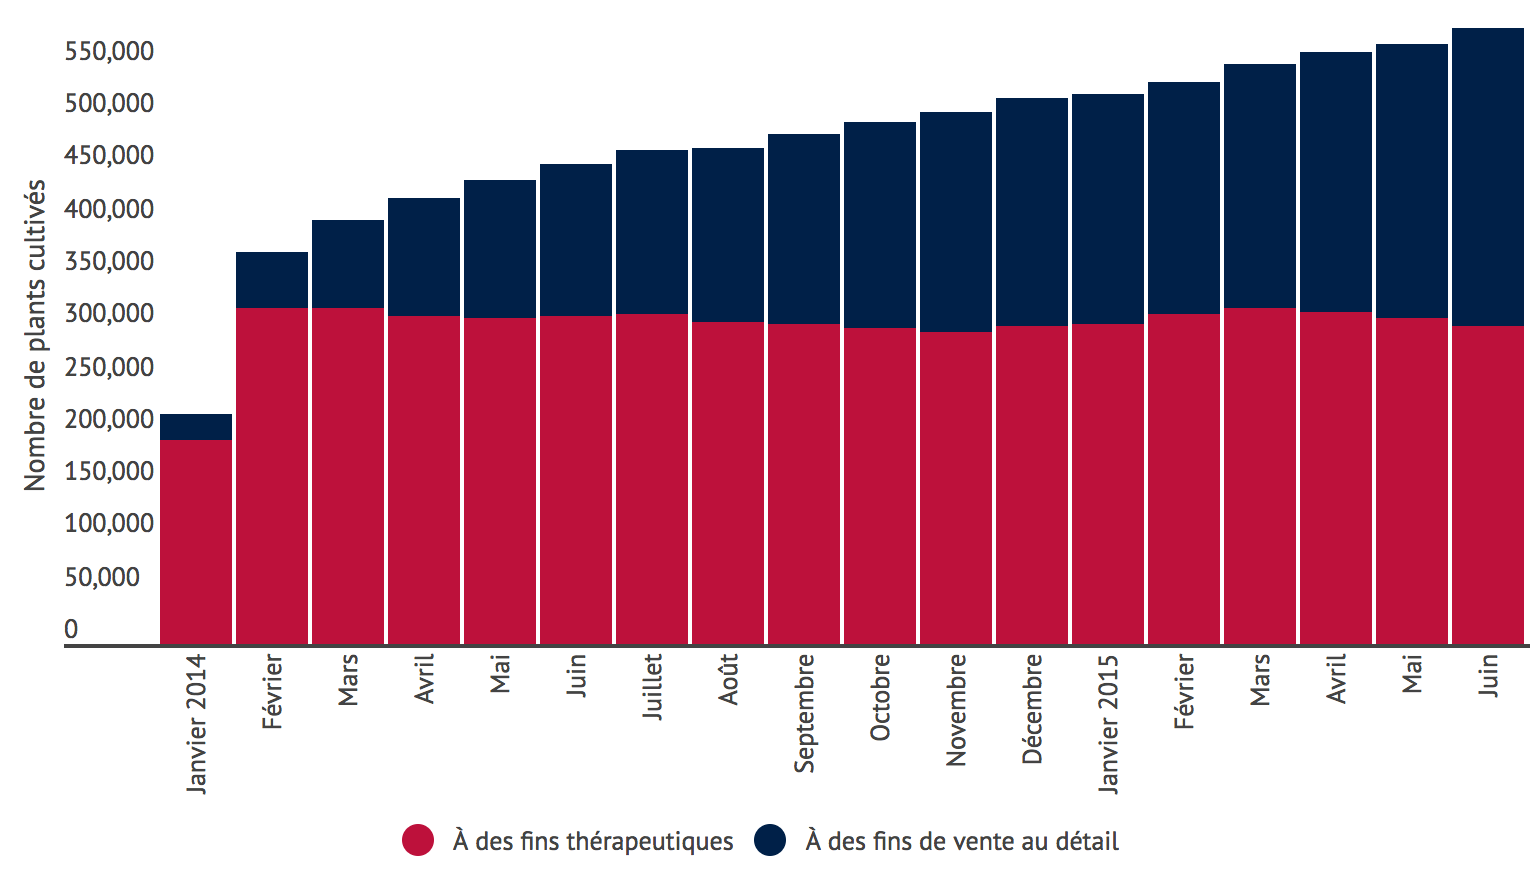
\includegraphics[width=\textwidth]{images/grapheconso.png}
    \caption{Nombre de plants cultivés au Colorado depuis la légalisation en 2014}
    \label{fig:grapheconso}
\end{figure}


Par exemple sur le graphique \ref{fig:grapheconso}, nous voyons qu’au Colorado, depuis la légalisation, le nombre de plants cultivés ne cesse d’augmenter. Cependant il faut rester sur ses gardes avec ces chiffres, il est en effet logique que ce chiffre croisse, le marché du cannabis se mettant en place avec sa concurrence sans vouloir indiquer une augmentation de la consommation de cannabis. En conclusion, pour le moment, la légalisation du cannabis aux États-Unis est plutôt considérée comme étant une réussite.

\paragraph{Depuis 1976, les Pays-Bas ont une politique dite de tolérance dans ce domaine :}

\begin{figure}\centering
	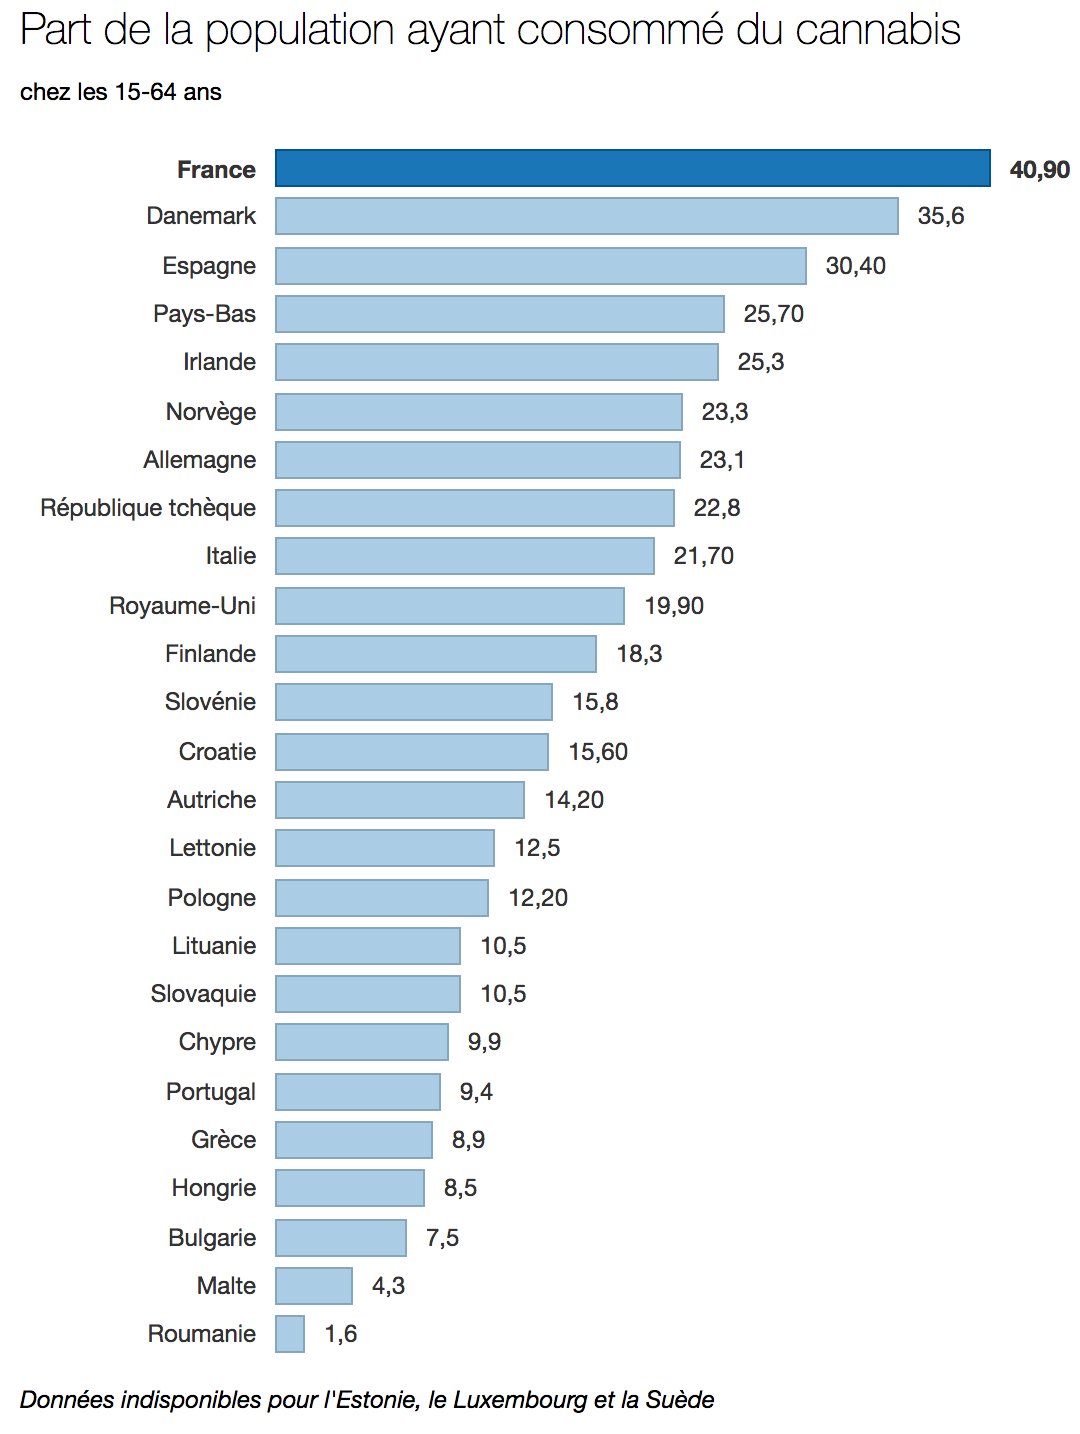
\includegraphics[height=.4\textheight]{images/grapheconsoPop.png}
    \caption{Part de la population ayant consommé du cannabis dans différents pays d'Europe}
    \label{fig:grapheconsopop}
\end{figure}

Enfin, un dernier élément va nous permettre de montrer que légaliser le cannabis peut permettre d’en éviter les abus. En effet, alors que la France est une des pays européens les plus répressif sur la question du haschich, nous voyons sur la figure \ref{fig:grapheconsopop} qu’elle est pourtant plus grande consommatrice que ses voisins. Comment expliquer qu’aux Pays-Bas, où le cannabis baigne dans une politique dite de tolérance depuis 1976, il y ait si « peu » de consommateurs ? Certes on dit que la pelouse est toujours plus verte chez notre voisin mais on peut quand même s'interroger sérieusement. Plusieurs raisons simples expliquent cela. Tout d’abord, le cannabis une fois autorisé est moins repoussant, moins tabou, il est donc plus facile d’éduquer la population sur le sujet et dès l’école. De plus, avec les revenus de la légalisation, il est possible d’être plus efficace sur la prévention, le système de santé, l’éducation etc. \cite{drugreport}

\section{Le cannabis, une bomb pour la santé ?}

Après avoir vu comment la légalisation du cannabis pouvait en influencer sa consommation, nous allons maintenant nous intéresser à la question de la santé. Une première interrogation se pose : est-il raisonnable de légaliser une substance qui peut affecter la santé ? Bien entendu, la réponse est non, en tous cas cela n’est pas plus raisonnable que de laisser légal et accessible de nombreuses autres drogues présente sur le marché qui ont, contrairement au cannabis bien plus la main rouge que la main verte.

\paragraph{Comparaison à des drogues légales}

En effet lorsque l’on regarde le bilan meurtrier de quelques substances qui nous sont bien familières, on se rend vite compte que le cannabis est en comparaison assez inoffensif. Dans le film-documentaire « The Union : the business behind getting high » de Brett Harvey, on apprend qu’en 2007 (année de sortie du film), aux États-Unis, les cachets de type aspirine ont provoqué la mort de 7500 personnes, le bilan du café s’élève lui à 10 000 victimes, vient ensuite l’alcool, responsable de  85 000 décès et enfin loin devant, nous retrouvons le tabac, meurtrier d’environ 450 000 personnes. C’est plus que les décès causés par le Sida, le crack, l’héroïne, les accidents de voiture, les meurtres, les incendies et l’alcool réunis. D’un autre côté, le docteur Lester Grinspoon nous apprend que depuis sa première utilisation par l’Homme, le cannabis n’a été relié à aucun décès (si l’on s’intéresse aux morts dûes à la substance seule). En effet il est pratiquement impossible pour l’Homme de faire une overdose suite à la consommation de marijuana, selon le docteur Paul Hornby, il faudrait fumer l’équivalent de 15 000 joints en à peine plus de 10 minutes pour risquer l’overdose. Ces chiffres son cependant à revoir à la baisse aujourd’hui, étant donné l’augmentation constante de la teneur en THC de la plante sur le marché noir. 

\paragraph{Les risques du cannabis :}

Vient ensuite la question du cancer, en effet la principale méthode de consommation du cannabis se fait par l’inhalation de fumée, cette méthode n’est-elle pas à risque ? Malheureusement, pour cette question, il nous est compliqué d’apporter une réponse, les études à ce sujet se contredisant énormément. Certaines nous disent que la fumée de cannabis contient dans une large mesure les mêmes substances cancérigènes que le tabac parfois en concentration plus forte, qu’en fumant du cannabis, on absorbe plus de monoxyde de carbone qu’en fumant du tabac, ou bien que le cannabinoïde méthandamide synthétique intensifie le développement des cellules du cancer du poumon et que la vaporisation prévient le dégagement de goudron et d’autres substances nocives et cancérogènes ---~c’est pourquoi il s’agit d’un des rares modes d’administration validé médicalement.\cite{cannacancer} 

Parallèlement, certaines publications scientifiques révèlent tout l’inverse, le cannabis n’aurait pas de lien avec le cancer de poumon, au contraire, l’inhalation de THC permettrait d’éliminer les potentielles cellules cancéreuses et donc de lutter contre le cancer. \cite{washington} Dans le film de Brett Harvey, le seul fait que de telles controverses existent est utilisé pour défendre le cannabis : « Si le cannabis avait un réel lien avec le déclenchement de cancer, ce dernier aurait été découvert depuis longtemps ».

Pour résumer le danger du cannabis en comparaison avec d’autres drogues nous pouvons utiliser les résultats du rapport sur la dangerosité des produits par le professeur Bernard Roques (table \ref{tab:drogues}).

\begin{table}\centering
	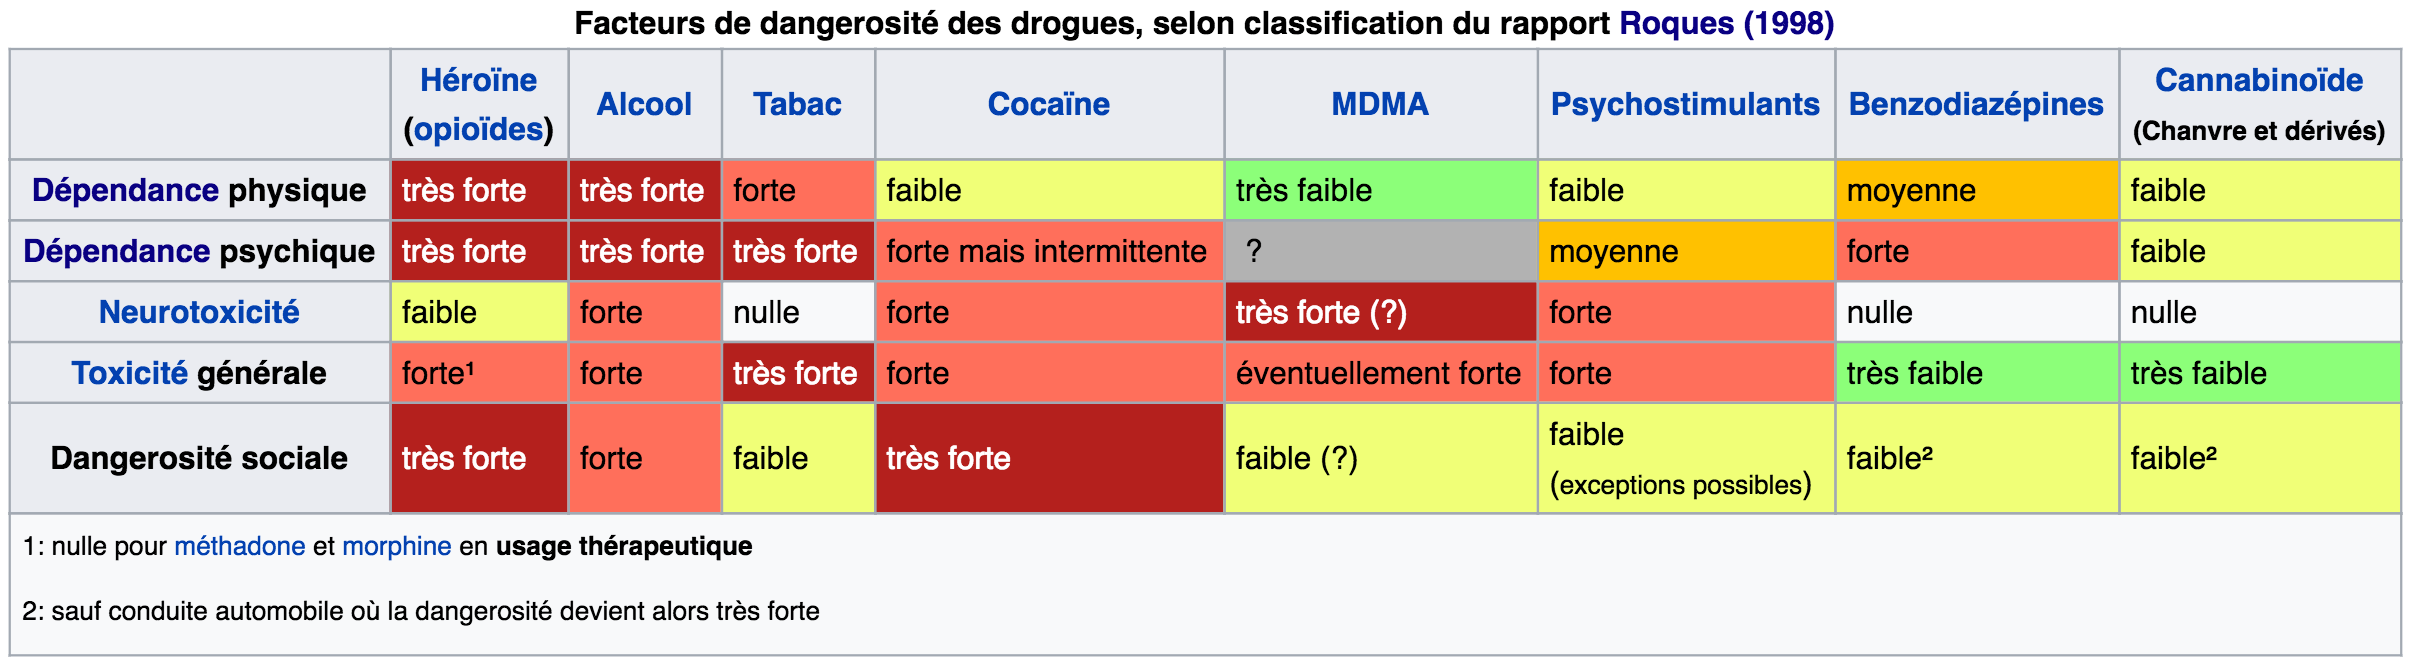
\includegraphics[width=\textwidth]{images/dependance.png}
    \caption{Comparaison des impacts sur la santé de différentes drogues}
    \label{tab:drogues}
\end{table}

   
Cependant selon Amine Benyamina, addictologue et président de la fédération française d’addictologie, il y a un réel danger liant le cannabis et la santé publique, qui concerne l’existence d’une population à risque. Cette population est constituée de deux groupes pour lesquels la consommation de cannabis est néfaste. Le premier est les jeunes, chez qui la  consommation peut nuire à la croissance du cerveau qui n’est pas encore achevée. Le second est constitué des personnes souffrant de troubles psychiatriques, dont un exemple souvent cité est celui de la schizophrénie. Le cannabis n’est pas responsable de cette maladie, en effet on peut remarquer que depuis plusieurs années la consommation de cannabis augmente tandis que le nombre de schizophrène reste lui constant, cependant il peut être responsable du déclenchement de la maladie chez les schizophrènes latents. \cite{franceCulture}).  Il est en même temps intéressant de savoir que le cannabis peut être utilisé comme anti-psychotique dans le traitement alternatif de certaines maladies psychotiques.   

\paragraph{Les bienfaits du cannabis :}

Nous pouvons donc maintenant nous demander quels sont les bienfaits du cannabis. Depuis plusieurs milliers d’années le cannabis est exploité pour nombre de ses caractéristiques (d’ailleurs, aux USA, la première loi qui a été faite sur le cannabis obligeait les fermiers à cultiver du chanvre).  Le chanvre est en effet une fibre très robuste et durable, il permet la fabrication de tissu, d’huile, de papier, et notamment, et c’est ce qui nous intéresse ici, la création de remèdes. Le cannabis a différentes propriétés médicinales : 
\begin{description}
	\item[Analgésiques] malades en phase terminale et pour les douleurs chroniques résistantes aux traitements traditionnels ; 
    \item[Relaxantes et somnifères] malades en phase terminale, troubles du sommeil ; 
    \item[Anti-spasmodiques] sclérose en plaques, épilepsie ; 
    \item[Anti-vomitives] traitement des effets secondaires de la chimiothérapie ou d'autres traitements lourds ;
    \item[Stimulant l'appétit et redonnant l'envie de manger] lutte contre la cachexie (maigreur extrême) et favorise la prise de poids ; 
    \item[Broncho-dilatatrices] asthme ; 
    \item[Anti-inflammatoires] le cannabidiol CBD non psychoactif est connu pour ses affinités avec les récepteurs CB2 situés sur les cellules immunitaires T;
    \item[Anti-psychotiques] traitement alternatif de la schizophrénie ; 	\item[Anti-dépresseur ;] 
    \item[Anxiolytiques ;]
    \item[Sédatives ;] 
    \item[Vasodilatatrices] glaucome, migraines ; 
    \item[Orexigènes] stimulation de l'appétit, en cas de maigreur importante ou de cachexie chez personnes âgées en long séjour, les patients atteint d'une maladie d'Alzheimer ou du sida ; 
    \item[Antalgiques] dans les cas de névralgie. 
\end{description}

Ses avantages naturels sont donc nombreux et intéressants pour la médecine, mais seul quelques médicaments à base de THC sont aujourd’hui présents sur le marché en France \cite{wikicannabismedical}. Pourtant ces remèdes à base de cannabis présentent de nombreux avantages : en plus d’être efficaces, ils sont ce qui se fait de plus naturel et ils sont surtout accessible à quiconque sait entretenir une plante. Une question se pose alors, pourquoi ces médicaments ne sont pas plus répandus? 

\paragraph{Le cannabis et ses mystères :}

Pourquoi la France garde-t-elle des réticences face à l’idée de laisser le chanvre libre sur son territoire sachant qu’à côté de cela elle n’en a aucune à être le troisième producteur mondial de morphine ? La France produit en effet 20\% du pavot légalement cultivé dans le monde, plante utilisé dans la médecine sous la forme de morphine mais aussi dans le milieu de la drogue sous l’appellation d’héroïne. Y a-t-il des enjeux derrière le sujet du cannabis ? 

  			\chapter*{Conclusion}
\addcontentsline{toc}{chapter}{Conclusion}

\section*{Retour d'expérience}

\subsection*{Choix du sujet, problèmes rencontrés et bilan}

Premièrement parti sur le sujet du système carcéral, le manque de réelle problématique, d’informations et simplement de motivation face au sujet nous on amené à revoir notre problématique de départ. Les recherches sur notre premier sujet nous avaient amené à aborder le cannabis, nous en avons finalement fait notre sujet d’étude. 

Ce thème s’est révélé fort intéressant, il nous a permis d’en apprendre beaucoup sur lui et de nous rendre compte de tout ce qu’il pouvait cacher. Mais ce sont notamment tous ses mystères qui ont rendu la réalisation de ce rapport compliquée. La recherche d’information sur le thème est difficile à cause des enjeux, des théories du complot, des blocages et des intérêts portés sur le cannabis. Beaucoup d’informations ne sont pas encore prouvées et il plane comme l’impression que rien n’est fait pour cela, ou bien encore qu’il est fait en sorte que cela reste ainsi. De plus c’est un sujet où il est difficile de trouver et surtout d’accepter des informations allant contre son avis de base, notre groupe n’est globalement pas contre la légalisation du cannabis, il est même plutôt en sa faveur, il nous fut donc difficile de rester subjectif. 

Au final nous en tirons le sentiment que la société se désinhibe peu à peu face au sujet du cannabis, des discussions et débats éclosent chaque jour, des évolutions sont observées. Il ne sera pas surprenant de voir le sujet du cannabis prendre de plus en plus de place dans les débats politiques de notre pays. Ils commencent déjà aujourd’hui même à faire parler de lui à l’approche des présidentielles de 2017, le 8 janvier 2017, 150 personnalités de Marseille demandent la "légalisation contrôlée" du cannabis.



\subsection*{Méthodes de travail}
Avant de rédiger notre monographie, nous avons collecté autant d’informations que possible autour du sujet du cannabis. La première difficulté fut de trier les informations à la fois utiles et fiables. Quand nous avons eu suffisamment d’informations pour avoir une problématique claire, chacun a choisi une partie puis l’a développé. Une fois que les trois parties furent rédigées, nous avons mis en commun notre travail pour être plus cohérents et ainsi éviter les répétitions. Enfin, nous avons fait la mise en page. Pour rendre le travail de chacun plus clair, nous aurions dû plus rapidement choisir le responsable de chaque partie afin de pouvoir mieux cibler nos recherches. De plus à ne vouloir se fermer aucune porte, nous avons surement dépensé trop d’énergie et de temps dans des recherches inutiles (pour le PSH).


\subsection*{Module PSH}

Nous avons apprécié, lors de ce module, d’être libres de choisir notre sujet ainsi que notre méthode de travail.

Cependant plusieurs demandes lors des séances dédiées aux modules (demande de plans, de listes de questions sur le sujet etc) nous ont détourné de nos recherches sur le sujet et ont été jugés assez peu utiles pour le bon fonctionnement de notre travail.

La découverte de nouveaux outils tel que Zotero fut cependant appréciée.








		\cleardoublepage 
   %     \nocite{*}
  %      \bibliographystyle{acm}
      \printbibliography
      
      
      \pagestyle{empty}
      \cleardoublepage~
      \newpage
      ~\vspace{5cm}
      \thispagestyle{empty}
      
      \begin{center}
      	\textbf{Abstract}
      \end{center}
Should France change its stance about recreational marijuana? The French government strictly enforces the repression of marijuana production, distribution, and consumption. This policy has a visible impact on society: on top of its prohibitive costs, social issues, such as criminality or prison overcrowding, may be consequences of the policy. We investigated to what extent these problems really are caused by the repressive governmental stance, and whether or not the country could benefit from a change of policy.

Many states already have more liberal legal frameworks for the use of marijuana. We used as our primary example that of the American state of Colorado, in which the consumption, growing and buying of marijuana has been legal for all citizens over 21 since 2014. We noted that the economic and social consequences of legalisation there were globally positive, considering for instance that criminality had dropped and some 10.000 to 18.000 jobs had been created. (related to marijuana?)

We also compared the current repression policy to the one enforced in the 1920s in the USA on alcohol. Indeed, the situation back then bears much resemblance to the current one: like alcohol, cannabis may induce dependence and cause health problems (which in the case of cannabis, is currently disputed by the scientific community). Moreover, prohibition makes ground in both cases for organised traffic and gang violence.
It appears that the legalisation on alcohol in the 1930s and on cannabis in Colorado, has greatly reduced criminality. Moreover, states have profited from legalisation, by being able to regulate the market and perceive taxes. However, these comparisons have made obvious the difference between depenalisation and legalisation, in a way we shall further explain in the full paper.


        
\end{document}